\documentclass[11pt]{article}

\usepackage[review]{acl}
\usepackage{times}
\usepackage{latexsym}
\usepackage[T1]{fontenc}
\usepackage[utf8]{inputenc}
\usepackage{microtype}
\usepackage{inconsolata}
\usepackage{graphicx}
\usepackage{amsmath,amssymb,amsthm}
\usepackage{booktabs}
\usepackage{xcolor}
\usepackage{tikz}
\usetikzlibrary{arrows.meta,positioning,fit}

\newtheorem{proposition}{Proposition}
\newtheorem{corollary}{Corollary}
\newcommand{\carve}{\textsc{Carve}}
\newcommand{\todo}[1]{\textcolor{red}{[TODO: #1]}}
\DeclareMathOperator*{\argmax}{arg\,max}


\title{When Is a Self-Improving Agent's Diagnosis Worth Verifying?\\Evidence Allocation When Every Check Costs an Episode}

\author{Anonymous ACL submission}

\begin{document}
\maketitle

\begin{abstract}
Self-improving LLM agents let an analyst model read failed trajectories, blame a component, and patch it. Because attributions are unreliable, recent systems verify a patch before applying it: they replay the failure with the patch, ask an LLM judge, or re-run tasks that used to pass. Methods for this step usually assume that some evidence is cheap. We measured it on three tool-use settings, a fault-injected customer-service environment and the retail and airline domains of $\tau^2$-bench, using over 14,000 agent runs and judge checks. Every kind of evidence costs about one episode: a single-step judge check costs 23--72\% of a full replay, and its sensitivity is only 0.37--0.57. We therefore recast verification as allocating a budget of episodes among targeted replays, null replays that measure spurious recovery, and regression runs, so as to maximise the net effect of the applied patches on success. A value-of-information argument shows that verification can pay only when a wrong patch does real harm: its value is bounded by $\min(\pi G,(1-\pi)H)$, where $\pi$ is the chance that the patch is right, $G$ its gain if right, and $H$ its harm if wrong. On $\tau^2$-bench, wrong patches almost never hurt: only 3 of 121 patches significantly raise failures on previously solved tasks. Consistent with the bound, applying every attributed patch without evidence is as good as any verification policy on held-out tasks (success 0.76$\to$0.88, against 0.83--0.88 for verified patch sets). When wrong changes carry a fixed cost, verification becomes useful, but no allocation policy dominates: the best one changes with domain and budget. A net-effect allocation that prices every experiment in episodes improves steadily with budget on both domains, whereas a multi-fidelity design method built on cheap checks degrades on airline as its budget grows. We release the environments, fault suites and intervention banks.
\end{abstract}

\section{Introduction}

A growing family of systems improves LLM agents from their own failures: the agent runs, an analyst model reads the failed trajectories, and its diagnosis drives a change to a prompt, a tool description or the orchestration \citep{shinn2023reflexion,zhao2024expel,hu2025adas,zhang2025dgm,agrawal2025gepa,chen2026harnessfix}. The diagnosis step, \emph{failure attribution}, is unreliable \citep{zhang2025whichagent,liu2026whowhenpro}: models label failures by their visible symptom rather than their cause, so a loop that trusts them will often change the wrong component. The common remedy is to verify before acting: patch the blamed component and replay the failure \citep{ma2025dover,lin2026reflect,shah2026car}, ask a judge whether the failing step is fixed, or re-run tasks that used to pass and keep the patch only if nothing breaks \citep{chen2026harnessfix}.

Verification costs agent episodes, so the natural research question is how to spend them. A tempting answer, and the one we started from, treats LLM judgements as cheap evidence and full replays as expensive, and allocates a budget across both by Bayesian experimental design. In a simulator built on these assumptions that approach needs half the budget of the strongest baseline (Appendix~\ref{app:carve}). On real agents the premise fails. Across three tool-use settings, a judge check costs 23--72\% of a full replay, because the judge must read the trajectory, and it detects only 37--57\% of real repairs. No evidence is cheap.

We therefore pose the problem with every piece of evidence priced in episodes, and ask a prior question: \emph{when is a diagnosis worth verifying at all?} Our contributions are:
\begin{itemize}
\setlength\itemsep{0pt}
\item A formulation of failure-driven self-improvement as \emph{episode-priced evidence allocation}. A patch's net effect on success decomposes into repair on its target category, spurious recovery that mimics repair, and regressions on other tasks; targeted replays, null replays and regression runs each estimate one term (\S\ref{sec:problem}).
\item A decision-theoretic bound: the value of verifying a patch is at most $\min(\pi G,(1-\pi)H)$, so verification pays only when a wrong patch is both likely and harmful. Together with the sample sizes needed to estimate each term, this yields a test practitioners can run before spending a budget on verification (\S\ref{sec:when}).
\item Measurements on ShopDesk and offline intervention banks on $\tau^2$-bench retail and airline, with paired replays and judge checks for every patch, null replays, and 20 regression runs for every patch any method accepts. Evaluating eleven policies against them shows that on these agents wrong patches are nearly harmless, and that applying attributed patches without evidence matches every verification policy on held-out tasks, as the bound predicts (\S\ref{sec:results}).
\item A net-effect allocation method that models the three terms with per-category spurious recovery and chooses experiments by knowledge gradient per unit cost. When wrong changes are costly, its gain grows steadily with budget on both domains, although no policy, ours included, is best everywhere (\S\ref{sec:method}, \S\ref{sec:results}).
\end{itemize}


\section{Related Work}

\paragraph{Failure attribution for LLM agents.}
\citet{zhang2025whichagent} introduced the Who\&When benchmark and compared all-at-once, step-by-step and binary-search prompting for locating the responsible agent and step; \citet{liu2026whowhenpro} extended it to longer and multimodal traces and found that attribution remains far from solved. AgenTracer uses counterfactual replay and fault injection to build training data for a small attribution model \citep{zhang2026agentracer}; AgentDebug pairs an error taxonomy with targeted corrective feedback \citep{zhu2025agentdebug}; ErrorProbe traces dependencies backwards and keeps a verified memory of error patterns \citep{li2026errorprobe}. Taxonomies such as MAST \citep{cemri2025mast} give attribution a fixed vocabulary, and AdaMAST induces a system-specific taxonomy from traces whose axes map to intervention points \citep{cemri2026adamast}. AdaMAST validates its taxonomy by agreement between LLM annotators; we instead treat the mapping from categories to components as a causal claim to be checked by intervention.

\paragraph{Verification by intervention.}
DoVer generates hypotheses from logs and validates each by editing a message or plan and re-running, with several runs per intervention \citep{ma2025dover}. REFLECT tests diagnosis-specific patches by targeted replay and feeds verified outcome changes back into attribution \citep{lin2026reflect}. CausalFlow scores steps by their causal responsibility under counterfactual interventions \citep{bonagiri2026causalflow}, and Causal Agent Replay formalises step interventions in a structural causal model with a point-of-commitment rule \citep{shah2026car}. AgentDebugX provides a toolkit with policy-gated reruns and a store of failure--diagnosis--repair bundles \citep{zhu2026agentdebugx}. All of these operate per trajectory or per hypothesis and do not decide how to allocate a shared budget across hypotheses, patches and levels of fidelity, which is our focus. Our method can use any of them as the replay primitive.

\paragraph{Self-improving agents.}
Reflexion, Self-Refine and ExpeL turn feedback into verbal lessons \citep{shinn2023reflexion,madaan2023selfrefine,zhao2024expel}; prompt optimisers such as ProTeGi, OPRO, TextGrad and DSPy use failures or textual feedback to rewrite prompts \citep{pryzant2023protegi,yang2024opro,yuksekgonul2025textgrad,khattab2024dspy}; ADAS, the Darwin G\"odel Machine and GEPA search over agent designs or prompts guided by evaluation and failure logs \citep{hu2025adas,zhang2025dgm,agrawal2025gepa}. HarnessFix attributes failures to harness artefacts, repairs them, and promotes a repaired harness only if it solves more validation tasks while breaking at most two \citep{chen2026harnessfix}; its validation is regression-aware, but it uses whole-task runs on fixed splits rather than allocating evidence per patch. Bayesian-Agent keeps Beta posteriors over the reliability of skills and applies threshold rules to patch, split or retire them \citep{wu2026bayesianagent}; its posterior is over skills rather than causal edges, and actions are chosen by fixed thresholds rather than by the value of information. \carve{} is complementary: it decides which proposed fixes to trust before they are applied.

\paragraph{Experimental design.}
Our selection rule is the KG(*) variant of the knowledge gradient \citep{frazier2008kg,frazier2010paradoxes}, within Bayesian experimental design \citep{chaloner1995bayesian}. Related problems include multi-fidelity bandits and optimisation \citep{kandasamy2016multifidelity,poloczek2017miso}, thresholding and best-arm identification \citep{locatelli2016thresholding,audibert2010bai,russo2016toptwo}, sequential testing \citep{wald1945sequential}, active causal structure learning \citep{tong2001active,hauser2014active} and causal bandits \citep{lattimore2016causal}. In software engineering, delta debugging isolates failure-inducing changes by experiment \citep{zeller2002dd}, and program-repair work warns that a patch passing a failing test may not fix the fault \citep{smith2015overfitting}, which our separation of edges from patch quality reflects. We use the knowledge gradient as an allocation rule, but our main question is a prior one from decision analysis: when the information is worth its cost at all.

\section{Problem: Episode-Priced Evidence}
\label{sec:problem}

\paragraph{Setting.} An agent is assembled from \emph{components} $j$ (prompt sections, tool descriptions, configuration). On a task distribution it fails with rate $F$; an LLM groups its failures into categories $i$ with shares $f_i$. For each \emph{cell} $(i,j)$ that the analyst blames, it proposes $K$ candidate patches $k$ that rewrite component $j$. Let $e_{ij}\in\{0,1\}$ indicate whether changing $j$ can repair category $i$ at all, and $q_k$ the fraction of category-$i$ failures that patch $k$ repairs if so. Separating $e$ from $q$ matters because a patch that fails to help may be aimed at the wrong component or merely be a bad patch.

\paragraph{Net effect.} Applying patch $k$ of cell $(i,j)$ changes the success rate by
\begin{equation}
\Delta_k \;=\; F f_i\, e_{ij}\, q_k \;-\; (1-F)\,\rho_k \;-\; c,
\label{eq:delta}
\end{equation}
where $\rho_k$ is the increase in failure rate on tasks that used to succeed (regressions, which may hit any category) and $c\ge0$ is a fixed cost of making a change (review, maintenance, risk), which we vary. The goal is to choose a set of patches that maximises $\sum_k\Delta_k$ on held-out tasks.\footnote{Effects of patches to different components are treated as additive; we check this assumption on held-out tasks in \S\ref{sec:results}.}

\paragraph{Evidence.} Three kinds of experiment, each costing a fraction of an episode, inform Eq.~\ref{eq:delta}:
\begin{itemize}
\setlength\itemsep{0pt}
\item A \emph{targeted replay} resumes a category-$i$ failure from the attributed step with the patch applied; it succeeds with probability $b_i+(1-b_i)e_{ij}q_k$.
\item A \emph{null replay} does the same without a patch and succeeds with probability $b_i$, the category's \emph{spurious recovery} rate. Without it, replay success cannot be interpreted.
\item A \emph{regression run} executes a previously successful task from scratch with the patch and fails with probability $r_0+\rho_k$, where $r_0$ is the natural re-run failure rate.
\end{itemize}
A fourth, a \emph{single-step check} that regenerates only the failing step and asks an LLM judge whether the error is gone, is often proposed as the cheap option. We measure its cost and accuracy in \S\ref{sec:results}. Unlike classic multi-fidelity settings, all four have costs within a factor of four of each other.

\section{When Can Verification Pay?}
\label{sec:when}

Consider one candidate patch. Before any evidence, let $\pi=P(e_{ij}{=}1)$ be the probability that it targets a real cause (for example, the analyst's audited accuracy), $G>0$ its expected net effect if it does, and $H\ge0$ its expected harm if it does not, so $H=(1-F)\bar\rho_{\mathrm{wrong}}+c$.

\begin{proposition}[Value of verification]
\label{prop:vpi}
With no evidence, the best action is to apply the patch iff $\pi G\ge(1-\pi)H$. The expected value of learning $e_{ij}$ exactly is
\begin{equation}
\mathrm{VPI}=\min\big(\pi G,\;(1-\pi)H\big),
\end{equation}
and any verification policy, which observes noisy outcomes instead of $e_{ij}$, gains at most this much.
\end{proposition}

The proof is two lines (Appendix~\ref{app:proofs}). The bound has a direct reading. When wrong patches are harmless ($H\approx0$), the default is to apply and verification has nothing to prevent; when the analyst is almost always right or almost always wrong, it has nothing to change. Verification is worth considering only when a patch is uncertain \emph{and} a wrong one does damage. The second ingredient is what the evidence costs.

\begin{proposition}[Cost of evidence]
\label{prop:cost}
Under Wald's approximations, a sequential test that decides $e_{ij}$ from targeted replays with error $\delta$ needs on average about $\log\frac{1-\delta}{\delta}\,/\,\mathrm{KL}\big(b+(1-b)q\,\Vert\, b\big)$ replays when the edge is real. Detecting a regression of size $\rho$ against a base rate $r_0$ with a one-sided level-$\alpha$ test and power $1-\beta$ needs about $(z_\alpha+z_\beta)^2 r_0(1-r_0)/\rho^2$ regression runs.
\end{proposition}

Two consequences follow. First, targeted replays are uninformative about $H$, because they only see the target category. A patch can pass every replay and still break other tasks, so verification that consists only of replays cannot capture the value in Proposition~\ref{prop:vpi} when $H$ comes from regressions. Second, small regressions are expensive to see. With $r_0=0.1$, a regression of $\rho=0.25$ is detected with 90\% power by 20 runs, whereas $\rho=0.03$ needs about 850. Verification is therefore most useful against rare, large harms, and it is the rate of such harms that decides whether it pays.

\section{Allocation Policies}
\label{sec:method}

When verification is warranted, the budget must still be allocated across cells, patches and experiment types. We compare eleven policies.

\paragraph{Net-effect allocation (ours).} We place a spike-and-slab model on each cell. The edge prior $P(e_{ij}{=}1)=\pi_{ij}$ comes from the analyst's attribution counts, shrunk towards a base rate by its audited accuracy (Eq.~\ref{eq:prior} in Appendix~\ref{app:carve}). Each $q_k$ has a grid posterior from a $\mathrm{Beta}(2,2)$ prior, each $b_i$ a Beta posterior updated by null replays, and each $\rho_k$ a Beta posterior updated by regression runs. Its estimate of Eq.~\ref{eq:delta} is $P(e_{ij}{=}1\mid\mathcal D)\,Ff_i\,\mathbb E[q_k\mid\mathcal D]-(1-F)\max(0,\mathbb E[r_k\mid\mathcal D]-r_0)-c$, where $r_k$ is the patch's failure rate in regression runs. The policy repeatedly runs the experiment (targeted replay of a patch, null replay of a category, or regression run of a patch) that maximises the $n$-step knowledge gradient of the decision value divided by its measured cost, with $n\in\{1,2,4,8\}$ \citep{frazier2008kg}, and finally applies every patch whose posterior net effect is positive. Unlike \carve{}, it has no single-step checks, a separate $b_i$ per category, and a regression term.

\paragraph{Baselines.} \emph{Apply attributed} uses no evidence: for each category it applies the first patch of the most-blamed component and of any component with at least 40\% of the blame. \emph{Replay-each} tests hypotheses in order of blame with three replays and accepts on two successes, as in do-then-verify methods \citep{ma2025dover}. \emph{HarnessFix-style, per patch} adds two regression runs that must break nothing; these counts are ours. \emph{HarnessFix-style, bundle gate} is closer to the original, which validates a whole bundle of repairs on held-out tasks and promotes it if it solves at least one more task and breaks at most two \citep{chen2026harnessfix}. We apply the \emph{Apply attributed} bundle, draw validation episodes from the bank, and allow three attempts. \emph{Uncertainty sampling} replays the cell with the largest frequency-weighted posterior uncertainty, with or without three cheap checks per patch first. \carve{} is our multi-fidelity design method (Appendix~\ref{app:carve}); we also run it with only full replays, with the judge's measured accuracy, and with a quality-dependent false-positive rate.

\begin{table*}[t]
\centering
\small
\setlength{\tabcolsep}{3.5pt}
\begin{tabular}{lcccccccccccc}
\toprule
 & \multicolumn{6}{c}{$\tau^2$ retail (development)} & \multicolumn{6}{c}{$\tau^2$ airline (held out)} \\
\cmidrule(lr){2-7}\cmidrule(lr){8-13}
 & \multicolumn{3}{c}{measured harm ($c{=}0$)} & \multicolumn{3}{c}{$+$ change cost $c$} & \multicolumn{3}{c}{measured harm ($c{=}0$)} & \multicolumn{3}{c}{$+$ change cost $c$} \\
Budget & 10 & 40 & 80 & 10 & 40 & 80 & 10 & 40 & 80 & 10 & 40 & 80 \\
\midrule
\csname @@input\endcsname tables/tau2.tex
\bottomrule
\end{tabular}
\caption{Net gain as a fraction of the oracle on the $\tau^2$ intervention banks, mean over 200 resampling seeds; bold is the best per column. ``Measured harm'' charges each accepted patch its significant measured regression; ``$+$ change cost'' also charges $c=0.02$ of the failure mass per wrong change. Standard errors are at most 0.08 (retail) and 0.03 (airline); they reflect resampling only, not the finite bank.}
\label{tab:tau2}
\end{table*}

\section{Environments and Intervention Banks}
\label{sec:setup}

\paragraph{Environments.} \emph{ShopDesk} is a customer-service environment we built, with a seeded database, six deterministic tools, exactly checkable answers and 11 named agent components. \emph{$\tau^2$-bench retail and airline} \citep{yao2024taubench,barres2025tau2} are dual-control customer-service domains with an LLM user simulator and database-state rewards. We split each domain policy into sections and add every tool description and the step limit as components, giving 24 components for retail and 21 for airline. The agent is DeepSeek-V4-Flash. Attribution, taxonomy induction \citep{wan2024tntllm}, patch generation and judging use DeepSeek-V4-Pro.

\paragraph{Faults that look like defects.} Each training episode runs clean or with one injected fault, written as a plausible authoring mistake rather than an obvious artefact. In retail: a policy section allowing gift-card refunds, a cancellation rule without the reason check, a product-tool description that confuses item and product ids, and a tight step limit. In airline: a wrong bag allowance, a 7-day instead of 24-hour cancellation window, a missing basic-economy restriction, proactive compensation, and a tight step limit. Clean episodes contribute natural failures: 22 of 137 on retail and 28 of 112 on airline.

\paragraph{Banks.} For each $\tau^2$ domain we take the 36 most-blamed (category, component) cells and generate three patches per cell. For every patch we record 20 paired targeted replays and single-step checks. We also record 20 null replays per category and 4 regression runs per patch, extended to 20 for every patch that any policy accepts (121 patches). Policies run offline by sampling outcomes from the bank, with costs in measured tokens and full replay $=1$, over 200 seeds. \emph{Ground truth needs no injected label}: an edge is real if its best patch's replay success exceeds the category's null rate by at least 0.2 (one-sided Fisher $p<0.05$), and a patch counts as regressing if its failure rate on previously solved tasks exceeds $r_0$ (one-sided binomial $p<0.05$). This yields 4 real edges on retail and 7 on airline. We report net gain (Eq.~\ref{eq:delta}) as a fraction of the oracle that applies exactly the real edges' best patches. We also apply the accepted patch sets to 40 unseen retail tasks.

\paragraph{Protocol.} Retail was the development domain for every method, including the variants in Appendix~\ref{app:dev}. Airline was evaluated once for the original policies and once, later, for the net-effect method, which was frozen on retail beforehand.


\section{Results}
\label{sec:results}

\subsection{What evidence costs and what it shows}

\begin{table}[t]
\centering
\small
\setlength{\tabcolsep}{3pt}
\begin{tabular}{lccc}
\toprule
 & ShopDesk & Retail & Airline \\
\midrule
Analyst accuracy $\hat r$ & 0.72 & 0.41 & 0.29 \\
Real edges among blamed cells & -- & 0.18 & 0.33 \\
\midrule
Judge check: cost / replay & 0.72 & 0.28 & 0.23 \\
\quad sensitivity & 0.57 & 0.37 & 0.41 \\
\quad false-positive rate & 0.21 & 0.11 & 0.13 \\
\quad break-even cost ratio & 0.08--0.13 & 0.09 & 0.10 \\
\midrule
Spurious recovery $b$ (mean) & -- & 0.23 & 0.20 \\
\quad range over categories & -- & 0--0.50 & 0--0.50 \\
Repair $q$ of real edges (median) & -- & 0.50 & 0.41 \\
Replays to decide an edge (Prop.~\ref{prop:cost}) & -- & 5 & 7 \\
\midrule
Natural re-run failure $r_0$ & -- & 0.11 & 0.14 \\
Patches regressing ($p{<}0.05$) & -- & 2/61 & 1/60 \\
Excess failure, wrong patches & -- & $+0.03$ & $-0.03$ \\
\bottomrule
\end{tabular}
\caption{Measured quantities. ``Real edges among blamed cells'' is the precision of applying every attributed patch. The break-even cost ratio is the cost below which judge checks are more informative per unit cost than replays (Appendix~\ref{app:carve}). Excess failure is relative to $r_0$; both have a standard error of about 0.01, and $r_0$ itself is uncertain by 0.03--0.04.}
\label{tab:measured}
\end{table}

Table~\ref{tab:measured} reports the quantities that Propositions~\ref{prop:vpi} and~\ref{prop:cost} depend on.

\paragraph{No evidence is cheap.} A judge check costs 23--72\% of a full replay, because the judge reads the trajectory, and it recognises only 37--57\% of real repairs. Its information per unit cost is below that of a replay in every environment: the break-even cost ratio is about 0.1, and the measured ratio is 0.23 or more. Its false-positive rate is no higher for bad patches than for good ones, so the failure mode we feared, a judge fooled by plausible bad patches, did not occur. The judge is weak, not misled.

\paragraph{Replays need controls.} Without any patch, 20--23\% of replays from the failing step succeed anyway, and the rate ranges from 0 to 0.5 across categories. A replay success rate of 0.5 is strong evidence in one category and none in another. Deciding one edge takes 5--7 replays even with the right $b_i$.

\paragraph{Wrong patches are nearly harmless.} With 20 regression runs per patch, only 3 of 121 patches raise failures on previously solved tasks significantly, about what chance alone would produce at $p<0.05$. On average, wrong patches change that failure rate by $+0.03$ on retail and $-0.03$ on airline, within the uncertainty of $r_0$. The exception we observed is on ShopDesk: a formatting patch (``reply \texttt{FINAL: N/A} rather than guessing'') made 26\% of held-out tasks answer N/A; removing it raises held-out success from 0.73 to 0.89. It passed its target-category replays, which by construction cannot see such harm (\S\ref{sec:when}).

\subsection{Does verification pay?}

Plugging the measurements into Proposition~\ref{prop:vpi}: with $H\approx0$, the value of verifying a blamed patch is close to zero, so the best policy should be to apply what the analyst blames. Two independent measurements agree.

\begin{table}[t]
\centering
\small
\setlength{\tabcolsep}{3pt}
\begin{tabular}{lcc}
\toprule
Patches chosen at budget 10 & Success & \#patches \\
\midrule
\csname @@input\endcsname tables/heldout.tex
\bottomrule
\end{tabular}
\caption{Held-out success on retail: 40 unseen tasks $\times$ 3 episodes (clean and fault-injected, as in training) with each policy's accepted patches, mean $\pm$ s.e.\ over 5 seeds. Episode noise is about $\pm$0.03 per patch set.}
\label{tab:heldout}
\end{table}

\paragraph{Held-out tasks.} Table~\ref{tab:heldout} applies each policy's patch set to 40 unseen retail tasks. Every set lifts success from 0.76 to 0.83--0.88, and applying the attributed patches without any evidence is among the best (0.88 with seven patches, most of them aimed at wrong edges). The verified sets are smaller and no better. Most of the gain comes from one patch, the step-limit fix, which almost every policy accepts.

\paragraph{Intervention banks.} The left half of each block in Table~\ref{tab:tau2} charges only measured regressions ($c=0$). Applying the attributed patches recovers 84\% (retail) and 60\% (airline) of the oracle's gain with no budget; no verification policy reaches it at any budget, because each rejects some real edges whose replays it cannot distinguish from spurious recovery within the budget. This is the regime of Proposition~\ref{prop:vpi} with $H\approx0$: rejecting a real edge costs gain, while accepting a wrong one costs nothing.


\subsection{When wrong changes cost something}

A deployment may still attach a cost to every change, for review, maintenance or risk that 20 regression runs cannot see. The right half of each block in Table~\ref{tab:tau2} charges $c=0.02$ of the failure mass per wrong change. Applying everything now drops to 16\% and 15\%, as its eight or nine wrong patches are charged, and verification pays. Which policy is best now depends on domain and budget. On retail, the per-patch HarnessFix-style rule wins at budgets 10 and 40 (0.52, 0.39) because the most valuable edge is also the most blamed, so testing in order of blame finds it at once; the net-effect method is best at 80 (0.50). On airline, \carve{} leads at budget 10 (0.30), HarnessFix-style at 40 (0.37), and uncertainty sampling with checks at 80 (0.35, against 0.33 for the net-effect method).

Two patterns are robust. The net-effect method improves with budget on both domains (retail 0.02$\to$0.50, airline 0.10$\to$0.33), whereas \carve{} \emph{declines} on airline (0.30$\to$0.19): with one shared spurious-recovery rate, further replays in high-$b$ categories push it to reject real edges. Second, cheap checks earn their place only by accident. With its default, overconfident check model, \carve{} beats its full-replay variant, but with the measured accuracy it runs almost no checks and stays close to its full-replay variant. The bundle gate that is closest to HarnessFix's own protocol is the weakest verifier under a change cost ($-0.36$ to $0.12$). It validates the analyst's whole bundle, so one real fix lets several wrong ones through.

\subsection{Why the simulator was optimistic}

Our first design study used a simulator in which \carve{} needed half the budget of the strongest baseline (Appendix~\ref{app:carve}). Re-running it with the measured judge accuracy, spurious recovery, analyst accuracy and cost ratio still predicts that \carve{} leads uncertainty sampling by 14 points on retail at budget 50. On the bank, the comparable variant (\carve{} with the measured check, scored with the change cost and without regressions) trails it by 15 points at budget 40. The simulator shared the method's structure: one $b$ for all categories, value spread over many edges, and a fixed regression cost $c$ that made every wrong change harmful. The last assumption alone decides whether verification pays (Proposition~\ref{prop:vpi}), and it was never measured.

\section{Discussion}

\paragraph{Measure $H$ first.} The bound in Proposition~\ref{prop:vpi} makes the harm of a wrong patch the first quantity to measure, before choosing a verification method. Measuring it needs regression runs, not targeted replays or judges, and with $r_0\approx0.1$ about 20 runs per patch reveal harms of 0.25 or more. On our agents such harms were rare, and verification policies mostly removed real fixes. Where wrong changes are costly (production agents, safety-relevant behaviour, changes reviewed by people), verification pays, and allocation matters.

\paragraph{Recommendations.} (i) Price every kind of evidence in measured tokens; judge checks were never cheap enough to help. (ii) Run null replays per category before interpreting replay success. (iii) Spend regression runs on screening for large cross-category harms. (iv) If changes are cheap and rarely harmful, apply attributed patches and let the next round of failures correct them.

\section{Conclusion}
We set out to make verification of LLM failure attributions cheaper and found that, on real agents, no verification evidence is cheap and wrong patches rarely hurt. Treating evidence as episode-priced and asking what verification can be worth at all shows that its value is capped by the harm it prevents. On our three tool-use settings that harm was close to zero, and acting on attributions without evidence matched every verification policy. Verification pays when wrong changes are costly, and then the allocation policy matters, though no single policy is best everywhere. We release the environments, fault suites and banks so that verification methods can be judged against measured interventions rather than simulators.

\section*{Limitations}
We study one agent model and one analyst model on three customer-service settings. The banks have 36 cells per domain and only 4 and 7 real edges, so individual edges weigh heavily, and resampling standard errors understate the uncertainty of a finite bank. Ground truth is defined by tests on 20 replays and 20 regression runs, which cannot see small effects. Regressions smaller than about 0.1 are invisible at this sample size, yet could accumulate over many patches. Held-out success was measured on retail at budget 10 only, and the patch sets of the earlier policies were chosen before the regression runs were extended. Most failures come from injected faults written to resemble real defects; natural failures are 16--25\%. The net-effect method was developed on retail after we had seen airline results for the other policies, although not its own. Finally, replay from a failing step requires deterministic tools.

\section*{Ethics Statement}
Self-improving agents change their own behaviour without a person reviewing each change. Our finding that wrong patches were rarely harmful holds for the agents and tasks we studied and should not be read as licence to skip review elsewhere. The ShopDesk example shows a single patch silently breaking a quarter of tasks. Our environments use synthetic customer data only.

\bibliography{references}

\appendix


\section{Proofs}
\label{app:proofs}

\paragraph{Proposition~\ref{prop:vpi}.} Without evidence the expected value of applying is $\pi G-(1-\pi)H$ and of not applying is $0$, so the default value is $\max(\pi G-(1-\pi)H,0)$. Knowing $e_{ij}$, one applies iff $e_{ij}=1$, for expected value $\pi G$. The difference is $\pi G-\max(\pi G-(1-\pi)H,0)=\min(\pi G,(1-\pi)H)$. A verification policy observes outcomes that are a garbling of $e_{ij}$; by the data-processing property of decision value (Blackwell), its value is at most that of observing $e_{ij}$, before subtracting the cost of its experiments.

\paragraph{Proposition~\ref{prop:cost}.} The first part is Wald's approximation for a sequential probability ratio test between $p_1=b+(1-b)q$ and $p_0=b$: with thresholds $\pm\log\frac{1-\delta}{\delta}$, neglecting overshoot, the expected sample size under $p_1$ is the threshold divided by the per-observation drift $\mathrm{KL}(p_1\Vert p_0)$. The second is the normal-approximation sample size of a one-sided test of a binomial proportion, evaluated with the variance at $r_0$.

\section{Development Variants}
\label{app:dev}

On the retail bank we tried, before any airline evaluation of them:
\begin{itemize}
\setlength\itemsep{0pt}
\item \carve{} with two null replays per category before trusting its replays (per-category $b$);
\item \carve{} with a regression gate of two runs per accepted patch;
\item both combined;
\item an evidence rule that requires a positive likelihood ratio from data;
\item tempered and flat priors;
\item a Bayesian regression gate.
\end{itemize}
With control replays and the gate combined, \carve{} gained 0.68 and 0.60 of the oracle at budgets 10 and 20, above plain \carve{} (0.42, 0.48), but fell below it at 40 and 80 (0.47 vs.\ 0.57 and 0.56). It never beat the per-patch HarnessFix-style rule (0.72, 0.73). Post hoc on airline it was worse than plain \carve{} (0.19 vs.\ 0.31 at budget 10). The other variants were worse everywhere; the evidence rule and the Bayesian gate accepted almost nothing (gain $\le0.12$). These numbers use the fixed change cost $c$ without regressions and the bank before the regression runs were extended. The net-effect method of \S\ref{sec:method} was developed afterwards, on retail, from the diagnosis that \carve{} lacked per-category spurious recovery and evidence for regressions.

\section{ShopDesk Details}
\label{app:shopdesk}

ShopDesk has six deterministic tools (orders, products, policies, refunds), answers checked exactly (refund amounts, counts, totals), and five injected faults: a tool description misstating price units, a list tool whose description omits pagination, a format instruction that rounds to whole dollars, a planning instruction that skips the policy lookup, and a tight step limit. Over three seeds, the analyst's attribution accuracy on injected failures was 0.75, 0.64 and 0.77. ShopDesk was evaluated online, without a bank: each policy ran against the live agent with fault-based ground truth (an edge is real when at least 30\% of a category's failures come from that component's fault). Table~\ref{tab:real} reports edge F1 and held-out success.

\begin{table*}[t]
\centering
\small
\begin{tabular}{lcccccc}
\toprule
 & \multicolumn{4}{c}{Edge F1 at budget} & Held-out & Single \\
Method & 10 & 20 & 30 & 60 & success @60 & checks \\
\midrule
\csname @@input\endcsname tables/real.tex 
\bottomrule
\end{tabular}
\caption{ShopDesk (3 seeds, mean $\pm$ s.e.). Held-out success after applying the patches accepted at budget 60 to 120 held-out episodes.}
\label{tab:real}
\end{table*}

\section{The \carve{} Design Study}
\label{app:carve}

Our first approach treated judge checks as cheap and replays as expensive, and allocated a budget over both by Bayesian experimental design. We keep it here as the multi-fidelity method compared in \S\ref{sec:results}, together with the simulator in which it was developed. The simulator shares the method's structure. Its results show the method working under its own assumptions, and they are not evidence about real agents.

\paragraph{Calibrated simulation.} With the measured judge accuracy, spurious recovery, analyst accuracy and cost ratio, the simulator predicts that \carve{} runs no judge checks on ShopDesk and retail and only a few on airline, which matches the break-even analysis in Table~\ref{tab:measured}. For $\tau^2$ retail it predicts net gains at budget 50 of 0.51 for \carve{} and 0.38 for uncertainty sampling; for airline, 0.33 and 0.31; for ShopDesk, 0.81 and 0.79.

\subsection{Problem Formulation}
\label{app:cproblem}

\begin{figure}[t]
\centering
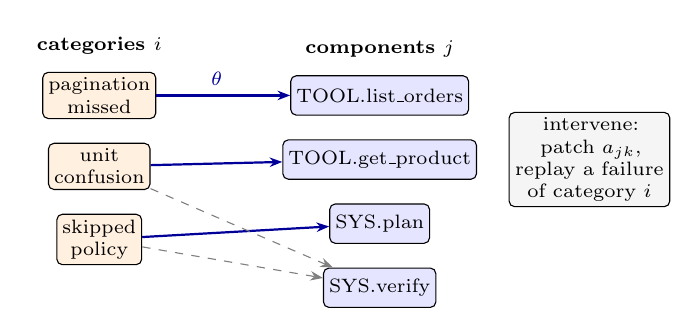
\begin{tikzpicture}[font=\scriptsize, node distance=3mm,
  box/.style={draw, rounded corners=2pt, align=center, inner sep=2pt, minimum height=5mm},
  cat/.style={box, fill=orange!12}, comp/.style={box, fill=blue!10},
  >={Stealth[length=1.6mm]}]
\node[cat] (c1) {pagination\\missed};
\node[cat, below=of c1] (c2) {unit\\confusion};
\node[cat, below=of c2] (c3) {skipped\\policy};
\node[comp, right=17mm of c1] (k1) {TOOL.list\_orders};
\node[comp, below=of k1] (k2) {TOOL.get\_product};
\node[comp, below=of k2] (k3) {SYS.plan};
\node[comp, below=of k3] (k4) {SYS.verify};
\draw[->, thick, blue!60!black] (c1) -- node[above, sloped, pos=.45]{$\theta$} (k1);
\draw[->, thick, blue!60!black] (c2) -- (k2);
\draw[->, thick, blue!60!black] (c3) -- (k3);
\draw[->, dashed, gray] (c2) -- (k4);
\draw[->, dashed, gray] (c3) -- (k4);
\node[above=1mm of c1, font=\scriptsize\bfseries] {categories $i$};
\node[above=1mm of k1, font=\scriptsize\bfseries] {components $j$};
\node[box, right=4mm of k2, text width=19mm, fill=gray!8] (o) {intervene:\\patch $a_{jk}$,\\replay a failure\\of category $i$};
\end{tikzpicture}
\caption{The category--component graph. Solid edges are true causal edges; dashed ones are plausible but wrong attributions (e.g.\ blaming verification for a unit error). Each intervention patches one component and replays one failure.}
\label{fig:graph}
\end{figure}

An agent is built from \emph{components} $j\in\{1,\dots,J\}$: sections of its system prompt, tool descriptions, tool implementations, orchestration settings. Its failures have been grouped into \emph{categories} $i\in\{1,\dots,I\}$ by an LLM, with $f_i$ the share of failures in category $i$. For every cell $(i,j)$ an analyst LLM can propose $K$ candidate patches $a_{ijk}$ that rewrite component $j$ to address category $i$.

\paragraph{Interventions.} An intervention $(i,j,k,\phi)$ samples a failed trajectory labelled $i$, applies patch $a_{ijk}$, and observes a binary outcome at fidelity $\phi$. A \emph{full replay} ($\phi=F$) resumes the episode from the attributed failing step and records whether the task now succeeds. A \emph{single-step check} ($\phi=S$) regenerates only the failing step and asks a judge whether the diagnosed error is gone. They cost $c_F$ and $c_S\ll c_F$.

\paragraph{Edges and patch quality.} We write $e_{ij}\in\{0,1\}$ for whether component $j$ is a cause of category $i$, meaning some change to $j$ repairs a non-trivial fraction of its failures, and $q_{ijk}\in[0,1]$ for the repair probability of patch $k$ when $e_{ij}=1$. This separation matters because a negative replay outcome is ambiguous: either $j$ is the wrong component or $a_{ijk}$ is a bad patch. Testing several patches per cell resolves the ambiguity.

\paragraph{Objective.} After spending at most budget $B$, the method accepts a set of cells $\mathcal{A}$ and, for each, a patch $k^\star_{ij}$. Accepting a true edge repairs a fraction $q_{ijk^\star}$ of category $i$'s failures; accepting a false edge costs a regression $c_{\mathrm{fp}}$, reflecting that unnecessary changes perturb behaviour on tasks that used to succeed \citep{vasudev2026intervention}. We measure
\begin{equation}
\begin{aligned}
G(\mathcal{A}) = {}&\sum_i f_i\Big(1-\!\!\prod_{j\in\mathcal{A}_i^+}\!\!(1-q_{ijk^\star_{ij}})\Big)\\
&- c_{\mathrm{fp}}\,\big|\{(i,j)\in\mathcal{A}:e_{ij}=0\}\big|,
\end{aligned}
\label{eq:gain}
\end{equation}
where $\mathcal{A}_i^+=\{j:(i,j)\in\mathcal{A},\,e_{ij}=1\}$. This is the net failure mass repaired; we report it as a fraction of the oracle value obtained by accepting exactly the true edges with their best patches.


\subsection{\carve{}}
\label{app:cmethod}

\paragraph{Observation model}
For a trajectory labelled $i$ and patch $a_{ijk}$, the probability that a full replay succeeds is
\begin{equation}
p_{ijk} = \begin{cases} \lambda\, q_{ijk} + (1-\lambda)\, b & e_{ij}=1,\\ b & e_{ij}=0,\end{cases}
\end{equation}
where $b$ is the spurious recovery rate (stochastic re-generation sometimes succeeds regardless of the patch) and $\lambda$ is the accuracy of the category labels used to sample trajectories; a mislabelled trajectory is treated as unaffected by the patch. A single-step check returns $z=1$ with probability $s\,p+\epsilon\,(1-p)$, where $s$ and $\epsilon$ are the sensitivity and false-positive rate of the check relative to the full outcome. All four nuisance parameters can be estimated from a small calibration set on which both fidelities and a human audit are run.

\paragraph{Attribution-informed prior}
Let $n_{ij}$ be the number of failures in category $i$ that the analyst attributed to component $j$, and $\hat r$ the analyst's attribution accuracy estimated on a small audited sample. With $d$ the expected number of causal components per category and $\rho=d/J$ the base edge density, we set
\begin{equation}
\pi_{ij} = (1-\hat r)\,\rho + \hat r\,\min\!\big(1,\ d\, n_{ij}/n_i\big),
\label{eq:prior}
\end{equation}
so that an unreliable analyst ($\hat r\to0$) yields the flat prior $\rho$ and a reliable one concentrates mass on the components it names. Eq.~\ref{eq:prior} is a heuristic interpolation, not a calibrated model; with a larger audit, $\pi$ could instead be fitted by logistic regression on audited attributions. Patch quality has prior $q_{ijk}\sim\mathrm{Beta}(\alpha_q,\beta_q)$.

\paragraph{Posterior}
Cells are independent given the data. For each cell we keep the posterior log-odds of $e_{ij}$ and, for each patch, a posterior over $q_{ijk}$ on a fixed grid of $G=101$ points. With $\mathcal{D}_{ijk}$ the outcomes observed for patch $k$,
\begin{equation}
\begin{aligned}
\mathrm{logit}\,P(e_{ij}{=}1\mid\mathcal{D}) ={}& \mathrm{logit}\,\pi_{ij}\\
&+ \textstyle\sum_k \log\big(\bar L^{1}_{ijk}/L^{0}_{ijk}\big),
\end{aligned}
\end{equation}
where $\bar L^{1}_{ijk}=\int P(\mathcal{D}_{ijk}\mid q,e_{ij}{=}1)\,dP(q)$ is the marginal likelihood of patch $k$'s outcomes under a true edge and $L^{0}_{ijk}=P(\mathcal{D}_{ijk}\mid e_{ij}{=}0)$.
Every update multiplies one grid vector by a likelihood vector, so updates and look-aheads are vectorised dot products.

\paragraph{Selecting interventions}
The value of the current decision for cell $(i,j)$, with $P_{ij}$ its edge posterior and $\hat Q_{ij}=\max_k\mathbb{E}[q_{ijk}\mid\mathcal{D}]$, is
\begin{equation}
V_{ij} = \max\big(P_{ij}\,f_i\,\hat Q_{ij} - (1-P_{ij})\,c_{\mathrm{fp}},\ 0\big),
\end{equation}
the expected contribution of the cell to Eq.~\ref{eq:gain} under the Bayes decision (accept iff the first term is positive), treating cells as additive. Eq.~\ref{eq:gain} combines components of one category multiplicatively, so $V_{ij}$ slightly overstates the value of a second cause for an already repaired category; we accept this approximation because it keeps cells independent. For an action $a=(i,j,k,\phi)$ repeated $n$ times, let $V'_{ij}(s)$ be the value after observing $s$ successes. The $n$-step knowledge gradient is
\begin{equation}
\mathrm{KG}_n(a) = \sum_{s=0}^{n} P(s\mid\mathcal{D},a)\,V'_{ij}(s) - V_{ij},
\end{equation}
and \carve{} runs the action maximising
\begin{equation}
\mathrm{score}(a) = \max_{n\in\{1,2,4,8\}} \frac{\mathrm{KG}_n(a)}{n\,c_\phi}.
\label{eq:score}
\end{equation}
Looking ahead several observations matters because a single binary outcome often cannot flip a decision, in which case $\mathrm{KG}_1=0$ even for a valuable cell; maximising over $n$ is the standard remedy \citep{frazier2008kg}. Because cells are independent, only the observed cell's scores change after each outcome, so each step rescores one cell in $O(KG)$ time after an initial pass over all cells.

\paragraph{Decisions and stopping.} At any point the method accepts the cells whose current value is positive and applies, for each, the patch with the highest posterior mean quality. It stops early when no action has a score above a small threshold, i.e.\ when no remaining experiment is expected to be worth its cost.


\subsection{When Do Priors and Cheap Checks Help?}
\label{app:canalysis}

These results analyse an idealised per-cell sequential test, not \carve{}'s full policy; they explain which quantities govern the method's behaviour. We consider a single cell and a single patch with known success probabilities $p_1$ (true edge) and $p_0=b$, under a rule that stops when the posterior log-odds leaves $[-A,A]$, $A=\log\frac{1-\delta}{\delta}$. Let $D_1=\mathrm{KL}(p_1\Vert p_0)$ and $D_0=\mathrm{KL}(p_0\Vert p_1)$ be the expected log-likelihood-ratio drift per observation under each hypothesis. Proofs, which follow Wald's approximations \citep{wald1945sequential}, are in Appendix~\ref{app:cproofs}.

\begin{proposition}[Value of the LLM prior]
\label{prop:cprior}
Let $|\ell|<A$ and neglect overshoot and stopping at the wrong boundary (whose probability is approximately $\delta e^{-\ell}$ for a true edge and $\delta e^{\ell}$ for a false one). A cell with initial log-odds $\ell$ then needs $N_1(\ell)=(A-\ell)/D_1$ observations in expectation if it is a true edge and $N_0(\ell)=(A+\ell)/D_0$ if not. Replacing a flat prior $\ell_\rho$ by LLM-derived log-odds $\ell_{ij}$ saves, in expectation over cells,
\begin{equation}
\Delta = \frac{\rho\,\mathbb{E}[\delta\ell\mid e{=}1]}{D_1} - \frac{(1-\rho)\,\mathbb{E}[\delta\ell\mid e{=}0]}{D_0},
\end{equation}
with $\delta\ell=\ell_{ij}-\ell_\rho$,
observations per cell, which is positive exactly when the prior raises true edges more, relative to their base rate and drift, than it raises false ones.
\end{proposition}

Under Eq.~\ref{eq:prior}, $\ell_{ij}\to\ell_\rho$ as $\hat r\to0$, so $\Delta\to0$: a useless analyst costs nothing beyond the flat prior, whereas trusting its labels outright (LLM-only) makes permanent errors. A miscalibrated analyst can make $\Delta$ negative, but only by an amount linear in the log-odds shift, after which the evidence takes over. Appendix~\ref{app:prop1} compares these predictions with simulated sequential tests.

\begin{proposition}[Cheap checks]
\label{prop:cfid}
Let $D^S_e$ denote the drifts of single-step outcomes, $z\sim\mathrm{Bern}(s\,p_e+\epsilon(1-p_e))$. Under the same approximations, a test using only single-step checks reaches the stopping boundary at lower expected cost than one using only full replays if and only if
\begin{equation}
\frac{c_S}{c_F} < \frac{D^S_e}{D_e},
\end{equation}
where $e$ is the true state of the cell.
\end{proposition}

Since $e$ is unknown, the proposition gives a clear rule only when the cost ratio lies outside the interval spanned by the two critical ratios; inside it, which fidelity is better depends on the posterior, which is what \carve{}'s look-ahead weighs.

With our default parameters ($p_1=0.54$, $b=0.05$, $s=0.85$, $\epsilon=0.15$) the critical ratio is $0.31$ for true edges and $0.44$ for false ones; with a weak check ($s=0.65$, $\epsilon=0.35$) it falls to $0.05$--$0.08$. Section~\ref{app:cfid} tests both predictions.


\subsection{Controlled Experiments}
\label{app:csim}

Real agents do not reveal which component truly caused a failure, so we first evaluate in a testbed where the causal graph is known and the method's model is deliberately misspecified.

\paragraph{Setup}
\paragraph{Testbed.} Each world has $I=12$ categories with Zipfian frequencies, $J=20$ components and $K=3$ patches per cell. Every category has one or two true components and one \emph{decoy} component that wrong attributions prefer, mimicking symptom-level mislabelling. Patch quality is bimodal: with probability 0.3 a patch is bad ($q\sim\mathrm{Beta}(1,9)$), otherwise $q\sim\mathrm{Beta}(6,3)$. A trajectory sampled for category $i$ is mislabelled with probability $1-\lambda=0.2$, in which case it comes from another category (weighted by frequency) and is repaired only if \emph{its own} edge to $j$ exists, unlike the model's flat treatment of mislabelled traces. The analyst attributes 20 failures per category with accuracy $r=0.5$; wrong attributions go to the decoy with probability 0.6. The analyst's accuracy is estimated from an audit of 20 attributions. Costs are $c_F=1$, $c_S=0.1$, $c_{\mathrm{fp}}=0.02$, and $s=0.85$, $\epsilon=0.15$, $b=0.05$. Section~\ref{app:crobust} relaxes the assumptions the generator shares with the model. Full details are in Appendix~\ref{app:sim}.

\paragraph{Baselines.} \emph{LLM-only} accepts, for every category, the most-attributed component and any component holding at least 40\% of the attributions, with the first patch, i.e.\ it acts on an induced taxonomy without verification. \emph{Replay-each} tests attributed hypotheses in order of attribution count with three full replays of the first patch and accepts a hypothesis if at least two succeed, mirroring do-then-verify methods such as DoVer; \emph{Replay-each, 3 patches} gives each hypothesis two replays of each of three patches and accepts if any patch succeeds twice; \emph{Sequential-each} replays each hypothesis, cycling through patches, until \carve{}'s own posterior leaves $[0.05,0.95]$. Untested hypotheses fall back to LLM-only, except for Sequential-each, which uses the Bayes decision. \emph{Thompson sampling} samples $(e,q)$ from the posterior and replays the cell and patch with the largest sampled repair. \emph{Uncertainty sampling} replays the cell with the largest frequency-weighted uncertainty $f_i\min(P_{ij},1-P_{ij})$, cycling through patches, at full fidelity; \emph{Uncertainty + cheap checks} first runs three single-step checks per (cell, patch) and then confirms with full replays. All baselines except LLM-only and the Replay-each variants share \carve{}'s posterior and decision rule, so comparisons among them isolate the selection rule.

\paragraph{Metrics.} Net gain (Eq.~\ref{eq:gain}) as a fraction of the oracle, and edge F1. We report means and standard errors over 50 worlds for the main experiment and 30 for the others; all methods see the same worlds, so differences are paired.

\paragraph{Main results}

\begin{figure*}[t]
\centering
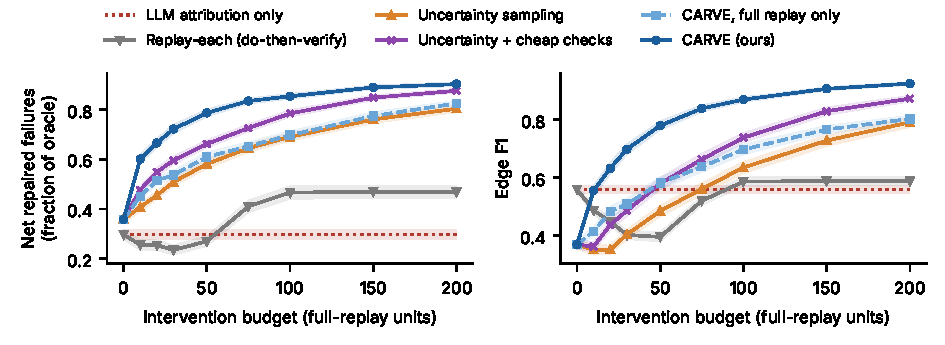
\includegraphics[width=0.85\textwidth]{figures/budget_curves.pdf}
\caption{Net repaired failure mass (left) and edge F1 (right) against intervention budget, 50 worlds, shaded $\pm1$ s.e.}
\label{fig:budget}
\end{figure*}

\begin{table}[t]
\centering
\small
\setlength{\tabcolsep}{3pt}
\resizebox{\columnwidth}{!}{%
\begin{tabular}{lcccc}
\toprule
 & \multicolumn{4}{c}{Budget (full-replay units)}\\
Method & 20 & 50 & 100 & 200 \\
\midrule
\csname @@input\endcsname tables/main.tex 
\bottomrule
\end{tabular}}
\caption{Net gain as a fraction of the oracle (mean $\pm$ s.e., 50 worlds). The lower block ablates \carve{}.}
\label{tab:main}
\end{table}

Figure~\ref{fig:budget} and Table~\ref{tab:main} show that \carve{} is best at every budget. With 50 units it recovers 79\% of the oracle gain; the strongest baseline, uncertainty sampling with the same cheap checks, recovers 66\% and needs about twice the budget (100 units, 78\%) to match it. The gap narrows at large budgets (90\% vs.\ 88\% at 200), as every reasonable method eventually resolves the frequent categories.

\paragraph{Where the gain comes from.} Two comparisons separate the selection rule from the cheap checks. With full replays only, \carve{} beats uncertainty sampling by 1--6 points (e.g.\ 0.609 vs.\ 0.581 at budget 50): the knowledge-gradient rule alone helps only modestly. Given cheap checks, its advantage grows to 7--13 points (0.787 vs.\ 0.662 at 50), because it decides per action whether a check is informative enough for its price and stops checking a cell once checks can no longer change the decision, whereas a fixed check-then-confirm schedule wastes checks on resolved cells. Most of \carve{}'s advantage is therefore in \emph{how it uses} cheap checks, which also makes their calibration critical (\S\ref{app:crobust}).

\paragraph{Verification baselines.} LLM-only is stuck at 30\% because it accepts decoys and bad first patches. Replay-each is initially \emph{worse} than not verifying: with $p_1\approx0.54$, requiring two successes in three replays rejects about 44\% of true edges even when the patch is good, and its fixed per-hypothesis cost exhausts small budgets on frequent but already-certain hypotheses. Testing three patches (61\% at 200) or stopping adaptively (81\% at 200) helps, but both remain well below \carve{} at small budgets (32\% and 52\% at 50). Thompson sampling spends most replays on cells it already believes in and reaches only 63\% at 200.

\paragraph{Ablations.} Removing single-step checks costs 15--18 points at small budgets. Restricting the look-ahead to one observation is below the full method at every budget and plateaus at 73\%, because many cells cannot be flipped by a single outcome and are never revisited. A flat prior costs 32 points at budget 20 and still 10 points at 200. With one patch per cell the method plateaus at 69\%: it cannot tell a wrong component from a bad patch and rejects true edges for good. Dropping the label-noise term makes no difference at the default label accuracy $\lambda=0.8$ (it is even slightly better at large budgets, 0.922 vs.\ 0.902 at 200), but it matters when labels are worse (\S\ref{app:crobust}).

\paragraph{When does the LLM prior help?}

\begin{figure}[t]
\centering
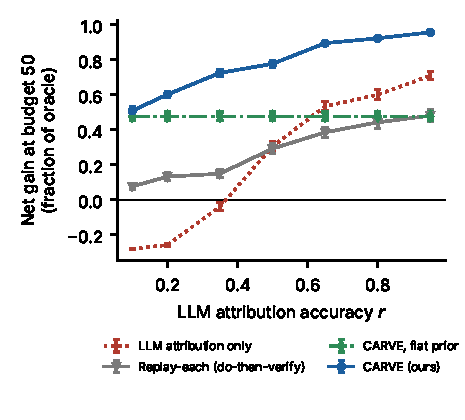
\includegraphics[width=\columnwidth]{figures/prior_sweep.pdf}
\caption{Net gain at budget 50 as the analyst's attribution accuracy $r$ varies (30 worlds, $\pm1$ s.e.).}
\label{fig:prior}
\end{figure}

Figure~\ref{fig:prior} varies the analyst's accuracy $r$. As Proposition~\ref{prop:cprior} suggests, \carve{} improves monotonically with $r$ and is never below the flat-prior variant: at $r=0.1$ it scores $0.51\pm0.02$ against $0.48\pm0.03$. The prior is not exactly flat there (the decoy still receives about twice the base rate), but its shifts are small, so evidence quickly dominates. Acting on attributions directly is harmful below $r\approx0.35$, where LLM-only has a \emph{negative} net gain (regressions outweigh repairs), and even at $r=0.95$ it reaches only 71\% of the oracle against 96\% for \carve{}, since it cannot detect bad patches. Replay-each improves with $r$ and only matches the flat-prior variant of \carve{} at $r=0.95$ ($0.48$ vs.\ $0.48$).

\paragraph{When do cheap checks help?}
\label{app:cfid}

Figure~\ref{fig:fid} (Appendix~\ref{app:extra}) is qualitatively consistent with Proposition~\ref{prop:cfid}. With the default check, the benefit of cheap checks shrinks as their cost grows and vanishes between 0.35 and 0.5 ($0.64\pm0.02$ vs.\ $0.61\pm0.03$ at 0.35, overlapping; $0.59$ vs.\ $0.61$ at 0.5), in line with the predicted critical ratios of 0.31 and 0.44. At cost 0.1, a check of quality $s-\epsilon=0.5$ (critical ratio 0.14--0.22) still helps, while one of quality 0.3 (critical ratio 0.05--0.08) brings no gain. At cost 0.5 \carve{} is slightly below its full-replay-only variant although its action set contains every full-replay action, which shows that the greedy rule is not exactly cost-optimal when the two fidelities are nearly equally efficient.

\paragraph{Robustness}
\label{app:crobust}

\begin{table}[t]
\centering
\small
\setlength{\tabcolsep}{3pt}
\resizebox{\columnwidth}{!}{%
\begin{tabular}{lcc}
\toprule
Condition (budget 50) & Unc.\ + checks & \carve{} \\
\midrule
\csname @@input\endcsname tables/stress.tex 
\bottomrule
\end{tabular}}
\caption{Violations of the model's assumptions (30 worlds). The judge-fooled row is the one setting where \carve{} loses.}
\label{tab:stress}
\end{table}

The generator shares several assumptions with the model: check errors depend only on the full outcome, cells are independent, the analyst's accuracy is estimated without bias, and the regression cost is small. Table~\ref{tab:stress} and Appendix~\ref{app:extra} relax each in turn.

\paragraph{Worse labels.} With label accuracy $\lambda=0.5$ both methods lose ground, and the label-noise term now matters: \carve{} scores 0.688, against 0.588 without the term and 0.513 for the baseline.

\paragraph{Biased analyst audit.} If the audit overstates the analyst's accuracy by 0.3, \carve{} actually improves (0.857), because a stronger prior concentrates the budget and the evidence corrects the decoys. Understating it by 0.3 costs 12 points (0.653), still above the baseline. Under-trusting a decent analyst is thus the more costly error in this testbed.

\paragraph{Regression cost.} Raising $c_{\mathrm{fp}}$ from 0.005 to 0.1 leaves \carve{} between 0.78 and 0.82, while LLM-only falls from 0.39 to $-0.13$: the more costly a wrong change, the more verification is worth.

\paragraph{Joint causes.} When 30\% of categories need two components changed together (a single patch then repairs only a fifth as often), violating cell independence, \carve{} drops from 0.787 to 0.661 at budget 50 but stays ahead of uncertainty sampling with checks (0.558; Table~\ref{tab:joint}).

\paragraph{Correlated check errors.} The one setting where \carve{} loses is when the single-step judge is fooled by plausible-looking bad patches (false-positive rate 0.6 for patches with $q<0.3$). \carve{} then trusts checks that systematically pass bad patches and falls to 0.377, below every method that relies on full replays (0.58--0.61). Modelling the dependence (a quality-dependent false-positive rate in the likelihood) restores it to 0.584, on par with full replays, at a cost of 9 points when the judge is not fooled (0.684 vs.\ 0.776). Whether real judges behave this way is therefore the most important quantity to measure before relying on cheap checks.

\paragraph{Nuisance parameters and scale.} Misspecifying $b$, $\lambda$ or the patch-quality prior changes the result by at most 5 points (Table~\ref{tab:misspec}, Appendix~\ref{app:extra}); misstating the check's sensitivity and false-positive rate costs 6--14 points. On a larger graph ($I=20$, $J=50$; Table~\ref{tab:scale}) the gap widens: at budget 50 \carve{} reaches 78\% of the oracle against 60\% for uncertainty sampling with checks.

\paragraph{Inside a self-improvement loop}

\begin{figure}[t]
\centering
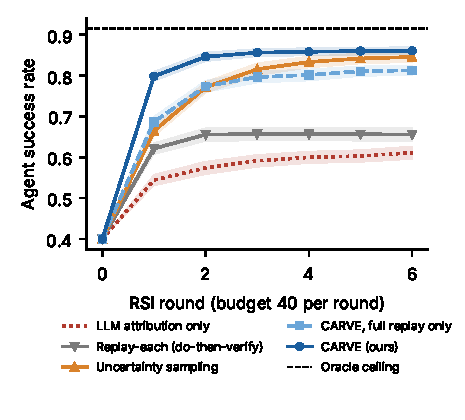
\includegraphics[width=\columnwidth]{figures/rsi.pdf}
\caption{Agent success over six rounds of attribute--verify--patch, with a budget of 40 units per round (30 worlds, $\pm1$ s.e.).}
\label{fig:rsi}
\end{figure}

Finally we embed each method in a loop. The agent starts at 40\% success. In each round the analyst attributes 240 new failures, sampled in proportion to the current failure distribution; the method spends 40 units; accepted patches are applied, which repairs failures (true edges) or adds a regression of $c_{\mathrm{fp}}$ times the current failure mass (false edges); and the failure distribution is recomputed, so priorities shift towards categories that remain. Posteriors carry over between rounds.

Figure~\ref{fig:rsi} shows that \carve{} reaches 80\% success after one round and 85\% after two, close to its plateau of 86\% (the oracle ceiling is 91.5\%). Uncertainty sampling with checks needs four rounds to reach 84\% and ends at 85\%; without checks it needs six. LLM-only and Replay-each plateau at 61\% and 66\%: once their accepted false edges and rejected true edges are fixed in place, new attributions do not correct them.


\subsection{Proofs for \carve{}'s propositions}
\label{app:cproofs}

\paragraph{Proposition~\ref{prop:cprior}.} Let $L_t=\ell+\sum_{u\le t}\log\frac{P(o_u\mid e=1)}{P(o_u\mid e=0)}$ be the posterior log-odds after $t$ observations. Under $e=1$, the increments are i.i.d.\ with mean $D_1=\mathrm{KL}(p_1\Vert p_0)>0$. The rule stops at $N=\inf\{t: L_t\notin(-A,A)\}$. By Wald's identity, $\mathbb{E}_1[L_N-\ell]=D_1\,\mathbb{E}_1[N]$. Wald's approximations give $P_1(L_N\le -A)\approx e^{-(A+\ell)}\approx\delta e^{-\ell}$ and $P_0(L_N\ge A)\approx\delta e^{\ell}$. Neglecting overshoot and this probability (which requires $\delta e^{|\ell|}\ll1$), $L_N=A$, hence $\mathbb{E}_1[N]=(A-\ell)/D_1$; if $\ell\ge A$ no observation is taken, which is why we assume $|\ell|<A$. Symmetrically, under $e=0$ the drift is $-D_0$ and $\mathbb{E}_0[N]=(A+\ell)/D_0$. Taking the difference between $\ell_\rho$ and $\ell_{ij}$ and averaging over cells with $P(e{=}1)=\rho$ gives $\Delta$. When the patch quality $q$ is unknown, outcomes are exchangeable rather than i.i.d.\ under the marginal likelihood, and Wald's identity does not apply directly; conditioning on $q$ recovers the result with $D_1=D_1(q)$, which approaches zero for a bad patch. This is the formal reason a single bad patch can stall verification and why \carve{} keeps several patches per cell.

\paragraph{Proposition~\ref{prop:cfid}.} By the same argument a single-step test needs $(A\mp\ell)/D^S_e$ observations at cost $c_S$ each, and a full-replay test needs $(A\mp\ell)/D_e$ at cost $c_F$. The single-step test is cheaper iff $c_S/D^S_e<c_F/D_e$. Since the single-step outcome is a garbling of the full outcome, the data-processing inequality gives $D^S_e\le D_e$, so the critical ratio is at most one.

\subsection{Simulation Details}
\label{app:sim}

Category frequencies are $f_i\propto 1/i$. For each category the number of true components is uniform on $\{1,2\}$ and the decoy is a further distinct component. The audit estimate $\hat r$ is a binomial proportion from 20 audited attributions. The prior uses $d=1.5$. The model's grid has 101 points; look-ahead horizons are $\{1,2,4,8\}$; the stopping threshold is $10^{-6}$. Replay-each uses three replays and accepts with at least two successes. Uncertainty sampling switches to an untried patch once the current patch has three full observations. In the loop experiment, 240 attributions per round are allocated to categories by a multinomial draw with the current failure distribution. All randomness is seeded; the code reproduces every number in this paper with \texttt{python -m sim.experiments all}.

\subsection{Checking Proposition 1}
\label{app:prop1}

Table~\ref{tab:prop1} compares the predicted expected number of observations with simulated sequential tests ($p_1=0.543$, $p_0=0.05$, $\delta=0.02$, 4000 runs per row). The predictions capture the direction and approximate size of the effect of the initial log-odds; they are least accurate when $|\ell|$ is large, where overshoot and wrong-boundary exits (last column) are no longer negligible.

\begin{table}[h]
\centering
\small
\begin{tabular}{rcccc}
\toprule
$\ell$ & $e$ & predicted $N$ & simulated $N$ & wrong exit \\
\midrule
\csname @@input\endcsname tables/prop1.tex 
\bottomrule
\end{tabular}
\caption{Proposition~\ref{prop:cprior}: predicted vs.\ simulated observations to a decision.}
\label{tab:prop1}
\end{table}

\subsection{Additional Results}
\label{app:extra}
\begin{figure}[t]
\centering
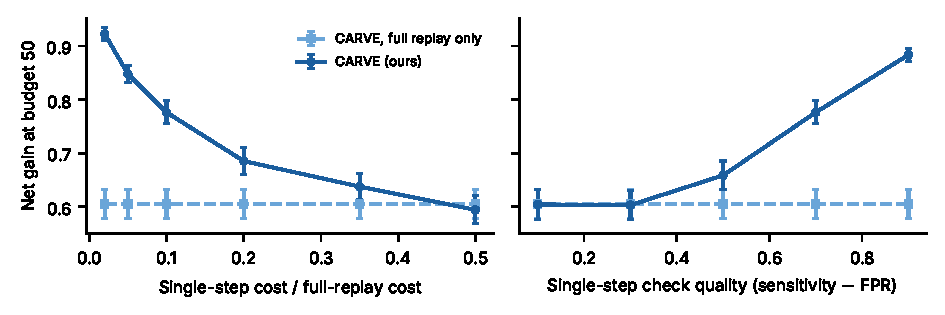
\includegraphics[width=\columnwidth]{figures/fidelity.pdf}
\caption{Effect of the single-step check's cost (left, quality fixed at $s{=}0.85$, $\epsilon{=}0.15$) and quality (right, cost fixed at 0.1) on net gain at budget 50.}
\label{fig:fid}
\end{figure}

\begin{table}[h]
\centering
\small
\setlength{\tabcolsep}{3pt}
\resizebox{\columnwidth}{!}{%
\begin{tabular}{lccc}
\toprule
Method & 50 & 100 & 300 \\
\midrule
\csname @@input\endcsname tables/scale.tex 
\bottomrule
\end{tabular}}
\caption{Net gain on a larger graph ($I{=}20$, $J{=}50$), 20 worlds.}
\label{tab:scale}
\end{table}

\begin{table}[h]
\centering
\small
\setlength{\tabcolsep}{3pt}
\resizebox{\columnwidth}{!}{%
\begin{tabular}{lcccc}
\toprule
Method & 20 & 50 & 100 & 200 \\
\midrule
\csname @@input\endcsname tables/joint.tex 
\bottomrule
\end{tabular}}
\caption{Net gain when 30\% of categories need two components changed together (30 worlds).}
\label{tab:joint}
\end{table}

\begin{table}[h]
\centering
\small
\begin{tabular}{lc}
\toprule
Model assumption (true value) & Net gain \\
\midrule
All nuisance parameters as in the generator & 0.776\,{\scriptsize$\pm$0.021}\\
Spurious rate $b$: 0.01 (0.05) & 0.811\,{\scriptsize$\pm$0.012}\\
Spurious rate $b$: 0.15 (0.05) & 0.826\,{\scriptsize$\pm$0.016}\\
Label accuracy $\lambda$: 1.0 (0.8) & 0.768\,{\scriptsize$\pm$0.022}\\
Label accuracy $\lambda$: 0.6 (0.8) & 0.794\,{\scriptsize$\pm$0.017}\\
Check $s/\epsilon$: .95/.05 (.85/.15) & 0.717\,{\scriptsize$\pm$0.016}\\
Check $s/\epsilon$: .70/.30 (.85/.15) & 0.636\,{\scriptsize$\pm$0.021}\\
Patch prior $\mathrm{Beta}(1,1)$ ($\mathrm{Beta}(2,2)$) & 0.811\,{\scriptsize$\pm$0.015}\\
Patch prior $\mathrm{Beta}(5,2)$ ($\mathrm{Beta}(2,2)$) & 0.777\,{\scriptsize$\pm$0.020}\\
\bottomrule
\end{tabular}
\caption{\carve{} with misspecified nuisance parameters, budget 50, 30 worlds. Several ``wrong'' values do slightly better than the generator's, a reminder that the model is misspecified in other ways too.}
\label{tab:misspec}
\end{table}



\end{document}
